\documentclass[11pt]{article}

\usepackage{url}
\usepackage{graphicx}
\usepackage{caption}
\usepackage{subcaption}

\begin{document}

\section{Introduction}

Web archiving initiatives generate vast amounts of data. The Internet Archive advertise their collection to be almost 2 petabytes, growing at a rate of 20 terabytes per month\footnotemark. As of October 2013 the British Library's archive of the UK web totalled 21 terabytes, growing by 4.5 terabytes over a one month period\footnotemark. The cost of providing storage for large collections can be high. For instance Amazon's Glacier service, an ``extremely low-cost storage service'', advertise storage rates of \$0.01 per GB per month as of February 2014. At this rate The Internet Archive would pay \$20,972 per month, the British Library would pay \$215. Requests to browse the archive would incur additional costs, as would expanding the archive. This situation motivates us to ask how web archive data can be compressed in order to optimally reduce storage space.

The Web ARChive (WARC) file format is the ISO standard\footnotemark commonly used to store web archive data. It is a plain text format that contains records of requests and responses of URLs, along with associated metadata, such as a list of links contained within the response data. The recommendation in the WARC standard is to append records to WARC files until they reach a size limit, at which point they should be gzipped and stored. The recommendation is that uncompressed WARC files should be no larger than one gigabyte. Using this recommendation our data set from Section~\ref{section:exp:github} compresses down to 17.469556\% of its original size. The WARC file format is extensible and the standard lists possible compression extensions. To our knowledge no such extension has been made publicly available and none are widely used. In this paper we explore possible extensions to the WARC format that would allow delta compression of consecutive records as well as different compression algorithms. We aim to: (i) reduce the total archive size and, (ii) allow easy partitioning of the database. The strategy that leads to the smallest total archive size compresses down to 11.883748\% of the original. Applying our strategy to the Internet Archive's collection would reduce their (hypothetical) Amazon Glacier costs to \$14,266 per month, a saving of \$6,706.

\footnotetext{\url{https://archive.org/about/faqs.php#9}}
\footnotetext{\url{https://web.archive.org/web/20131017144821/http://www.webarchive.org.uk/ukwa/statistics}}
\footnotetext{\url{http://www.iso.org/iso/catalogue_detail.htm?csnumber=44717}}

\section{Background}

\begin{enumerate}
\item WARC spec
\item gzip, bzip2, tar. What they do, why these ones?
\item vcdiff, bsdiff, diffe. What they do, why these ones?
\item internet archive, IIPC, BL. Collections, experience
\item Heritrix
\end{enumerate}

\section{Experiment: Generated Data}

\begin{enumerate}
\item generate 1MB text data
\item apply change repeatedly
\item compression strategy
\item compare
\item very many changes, over time. What wins
\item More than just text data? What kinds of changes?
\end{enumerate}

\section{Experiment: GitHub Pages}\label{section:exp:github}

The code hosting service GitHub\footnotemark offers a free service called GitHub Pages\footnotemark that allows users to host static web content for free. In order to evaluate different compression strategies on realistic data we conducted a crawl of GitHub Pages projects. These projects are stored in version control and so it is possible to iterate through the changes made to the files over time. This approximates the changes observed to web pages over time and so forms a suitable data set for compression comparison. There were 27,507 suitable projects as of November 2013. Of these projects, X did not contain suitable web documents.

\subsection{Data}

The data set is made up of projects hosted on GitHub that conform to the projectname.github.io naming scheme. GitHub treats these projects as GitHub Pages projects and serves their content at the URL given by the name. Before hosting, a project's files are processed by a static website generator called Jekyll\footnotemark. This software generates files from templates that use various markup languages, e.g. HTML, Markdown, or Liquid. When changes are pushed to the Git repository for the project the files and website are updated. To generate our data set we clone a project repository and iterate through every commit. For each commit we process the files using Jekyll and serve the results up locally. We then direct Heritrix to archive the site. When Heritrix has finished we stop serving and continue to the next commit.

During this process we have crawled 26 domains, discovering 1792 URIs. Heritrix sent 89,759 requests for pages and received 11,006 unique responses. This means that for every eight requests that Heritrix sent out only one returned content that had not been seen before. Our archived data spans 1829 days, starting 2008-10-19 running up to 2013-10-22.

% TODO: Using version control language, need to define? e.g. clone, push
% TODO: How many projects do not contain web documents.
%       We'll need to wait for Heritrix to process them
%       and then count the empty Heritrix jobs.
%       Currently 83 of 293 (28%)
%       Should we expect 7792 projects in total to be dead?

\footnotetext{\url{http://github.com/}}
\footnotetext{\url{http://pages.github.com/}}
\footnotetext{\url{http://jekyllrb.com/}}

\subsection{Compression Analysis}

We now explore different strategies for minimising the archive size using compression algorithms. We begin with the WARC files that Heritrix has produced. Before compressing we first ensure that any response records that contain identical content are replaced with revisit records with the identical payload profile. We also combine files under the same domain, limiting the total file size to 1 gigabyte, as recommended by the specification. We consider three different delta algorithms; diff, bsdiff, and vcdiff. For each algorithm we use three different strategies; delta from the first ever record, from the immediately preceding record, or from a reference frame stored every 10 records. When we apply a delta to a record we leave the WARC headers intact and we only consider records that are response records. We compare two compression algorithms; gzip and bzip2, we also consider tar files that use these compression types. When compressing, we treat each file individually, when using tar compression we consider all files under the same domain. Storage restraints meant that our experimental set up did not allows us to consider the archive as a whole, we instead consider each domain individually. This means that each WARC file that we consider contains only records from that domain. It also means that many WARC files do not reach the 1 gigabyte size limit. When creating a tar file we can only combine files from the same domain. We believe that this means that our compressed archive sizes are slightly larger than they would be in a production environment.

Figure~\ref{fig:tas_delta_compression} shows the total archive size for different compression and delta algorithm strategies. The WARC specification recommends that files are compressed using gzip, applying this strategy to our archive compresses the files down to $17.469556\%$ of the original. We see that applying a bzip2 algorithm would compress the archive down to $13.749876\%$ of the original. Figure~\ref{tas_delta_compression:b} shows the effect of applying delta algorithms to the data. The best performing delta strategy uses bsdiff to calculate the delta between each consecutive record. Using this strategy we see a $67.244168\%$ reduction in total archive size.

\begin{figure}
\centering
\begin{subfigure}{.5\textwidth}
  \centering
  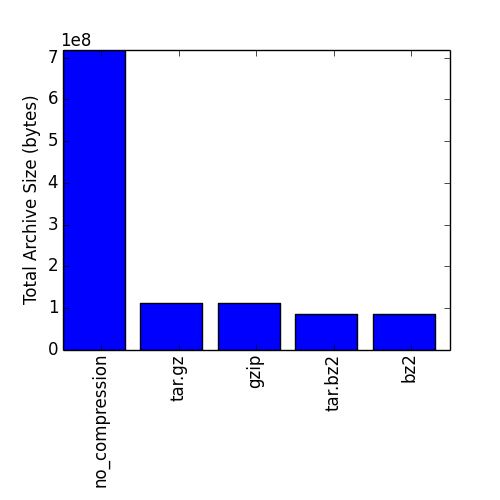
\includegraphics[width=\linewidth]{images/tas_compression.png}
  \caption{Compression comparison.}
\end{subfigure}%
\begin{subfigure}{.5\textwidth}
  \centering
  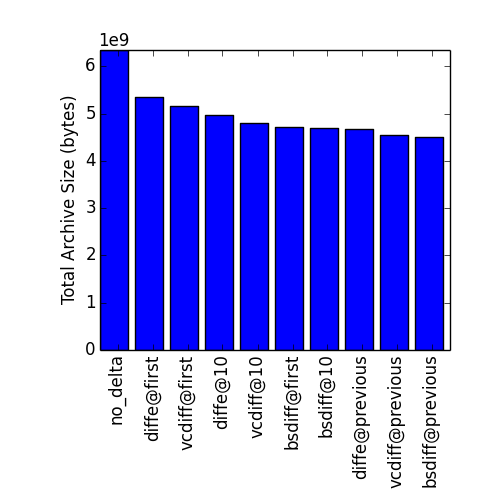
\includegraphics[width=\linewidth]{images/tas_delta.png}
  \caption{Delta comparison.}
  \label{fig:tas_delta_compression:b}
\end{subfigure}
\caption{Total archive size for different delta and compression strategies.}
\label{fig:tas_delta_compression}
\end{figure}

asd

\begin{figure}
  \centering
  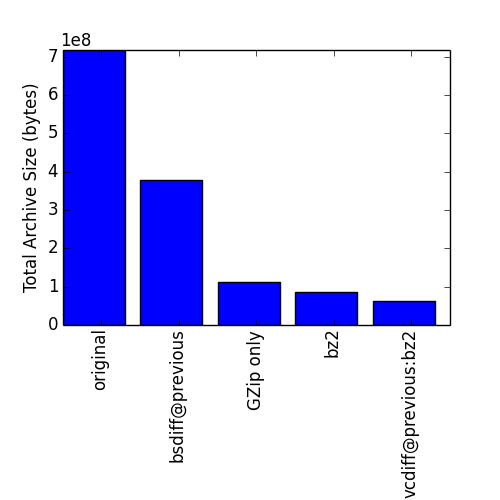
\includegraphics[width=\linewidth]{images/tas_best.png}
  \caption{Total archive size for different delta and compression strategies.}
  \label{fig:tas_best}
\end{figure}

\begin{enumerate}
\item without delta how does each compression algorithm compare?
\item which algorithm should be picked?
\item ignoring compression which delta algorithm performs the best?
\item which should be picked?
\item what is the best overall strategy?
\item what are the pros and cons of this strategy. e.g. speed, partitioning, do we gain little over the other strategies in terms of size but lose on speed?
\item additionally:
\begin{enumerate}
\item average size of warc record types, before and after.
\item counts of warc record types
\item percentage space taken up by each type
\item savings introduced by compression, why not compress the other types?
\item compression performance by content type
\item refer to content analysis for frequencies of content type. e.g. is it worth finding an algorithm that compresses images really well? or can we ignore them because HTML and its high change frequency trump image for storage issues.
\end{enumerate}
\end{enumerate}

\subsection{Content Analysis}

Figure~\ref{fig:commits_per_day} shows the number of changes made to all files in the archive per day. The data is split into two parts for clarity. The split is made on the day that GitHub pages launched their new naming scheme, projectname.github.io. Previously the naming scheme had been projectname.github.com. Our data crawl did not consider projects that had kept the old naming scheme, this is why the numbers increase. In the first 1658 days the average number of changes per day was 0, in the last 170 that increases to 58.

% Billy: I've held back on looking at these graphs in an detail because I think they will change quite a bit as I add more domains.
% TODO: Insert more meaningful analysis of change frequency. Is there a strong correlation? Can we say something like 'the average domain will update at least one page every X days'? DO we see an increase in change frequency over time? Is this explained by an increase in suitable projects over time? Can we correct for this?

\begin{figure}
\centering
\begin{subfigure}{.5\textwidth}
  \centering
  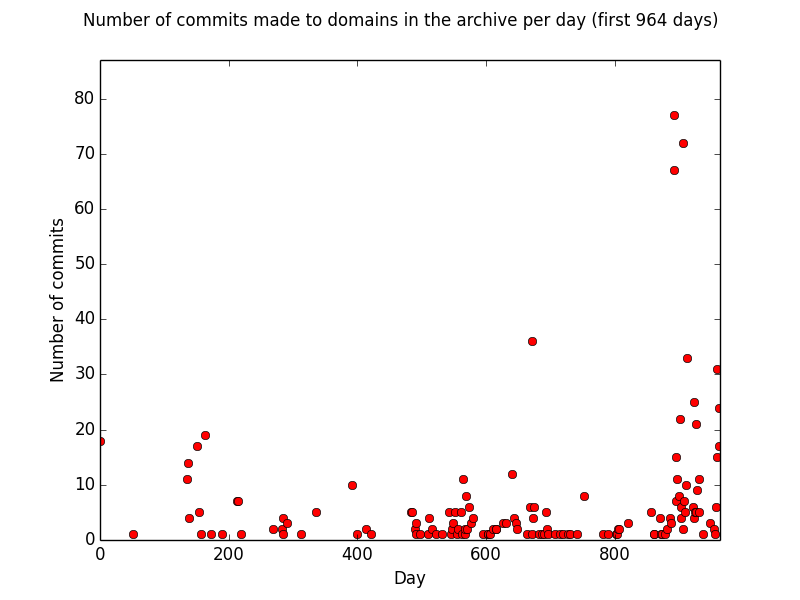
\includegraphics[width=\linewidth]{images/commits_per_day_first.png}
  \caption{During the first 1658 days.}
\end{subfigure}%
\begin{subfigure}{.5\textwidth}
  \centering
  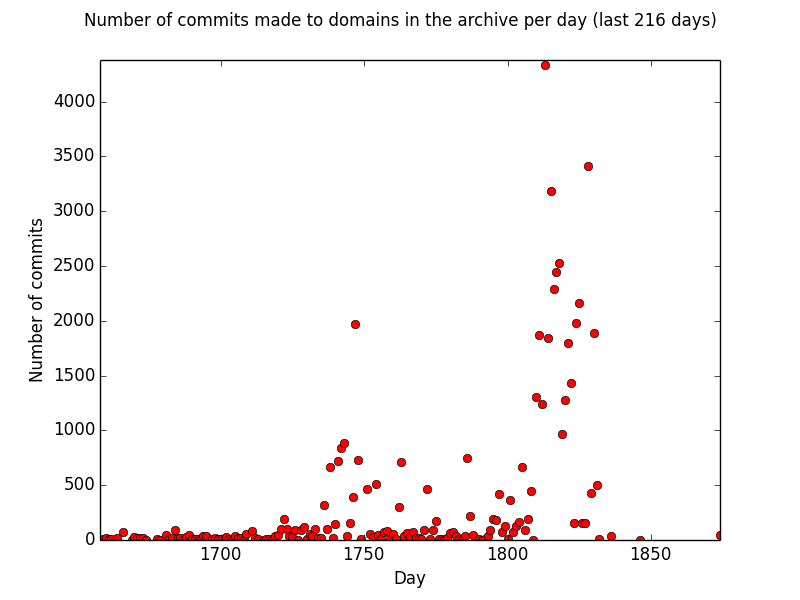
\includegraphics[width=\linewidth]{images/commits_per_day_last.png}
  \caption{During the last 171 days.}
\end{subfigure}
\caption{Number of commits made in the archive per day.}
\label{fig:commits_per_day}
\end{figure}

Each change above is an observation of a single file's contents differing from a previous crawl. This means that if a HTML file and a CSS file were updated simultaneously, we would record two changes. This might not align with an archivist's view of what a webpage change would be. Instead, they might expect to record a single change for updates made in a short period of time, no matter how many files were edited. In addition, we iterate through every commit made to the project but changes are only made public for every push. There may be several commits made to a project before a push. Considering this, we can instead assume that a maximum of one change is made to a domain per day. Figure~\ref{fig:changes_per_day} shows the updated number of changes made to the archive per day. During the first segment we expect to have a domain updated in the archive once every 12 days, in the second segment this is once every day.

% Billy: Again, I'll have to revisit this when I have more data. The first outlier in the first segment jumps to 14 domains changing in a single day. I looked into it and it's the result of a single developer creating 14 almost identical websites in one day. They're all for open source programmes run in US colleges. The other outliers I'm not sure about yet.

\begin{figure}
\centering
\begin{subfigure}{.5\textwidth}
  \centering
  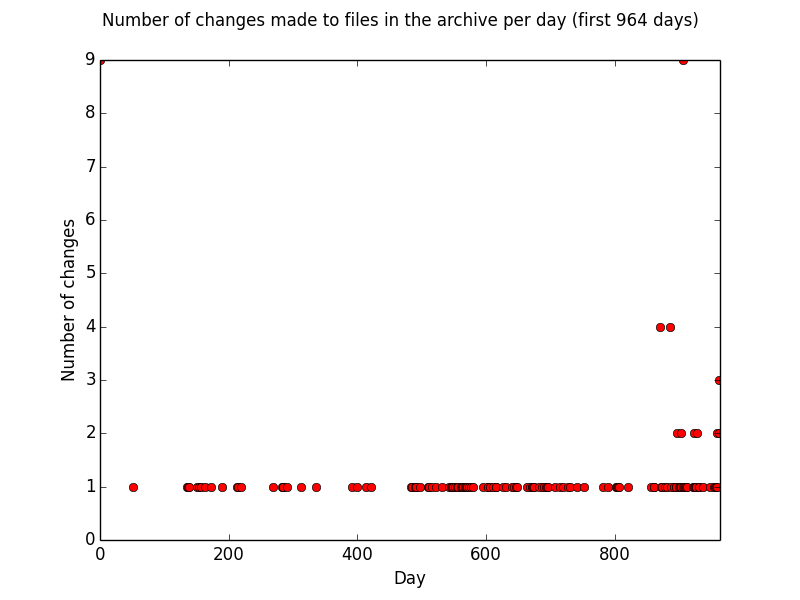
\includegraphics[width=\linewidth]{images/changes_per_day_first.png}
  \caption{During the first 1658 days.}
\end{subfigure}%
\begin{subfigure}{.5\textwidth}
  \centering
  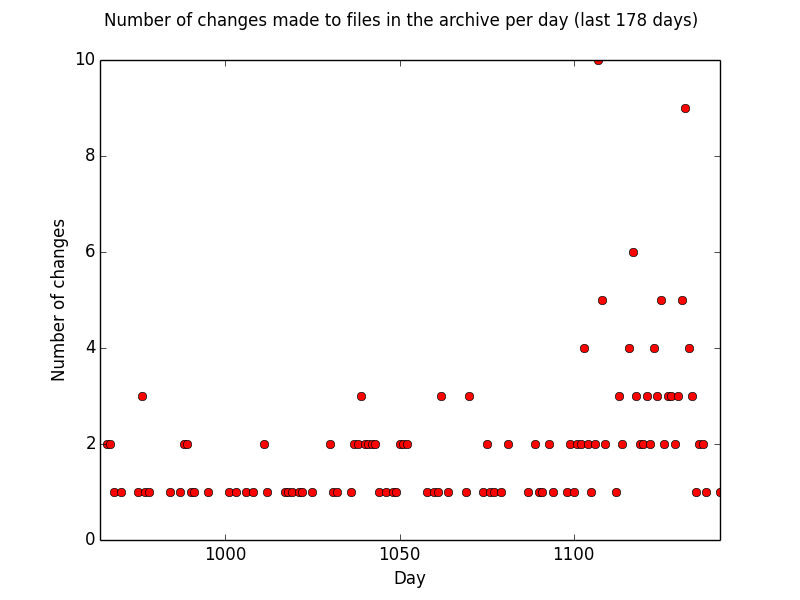
\includegraphics[width=\linewidth]{images/changes_per_day_last.png}
  \caption{During the last 171 days.}
\end{subfigure}
\caption{Number of changes made in the archive per day.}
\label{fig:changes_per_day}
\end{figure}

Figure~\ref{fig:uris_per_domain} shows the number of URIs observed in each domain. Figure~\ref{fig:uris_per_domain:a} shows the total number of URIs ever observed at a domain. Figure~\ref{fig:uris_per_domain:b} shows the average of the number of URIs observed at each domain over all crawls.

% Billy: Again, before doing proper analysis, let's get more data.
% Billy: It appears that domains have lost between 1/3 - 1/2 of their pages over time. If this trend persists, we might be able to come up with a confident lifetime for a URI. I don't anticipate this though, I thought that URIs were fairly stable, e.g. /index.html stays around for a very long time.

\begin{figure}
\centering
\begin{subfigure}{.5\textwidth}
  \centering
  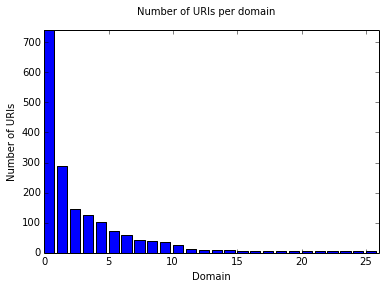
\includegraphics[width=\linewidth]{images/uris_per_domain.png}
  \caption{Total URIs.}
  \label{fig:uris_per_domain:a}
\end{subfigure}%
\begin{subfigure}{.5\textwidth}
  \centering
  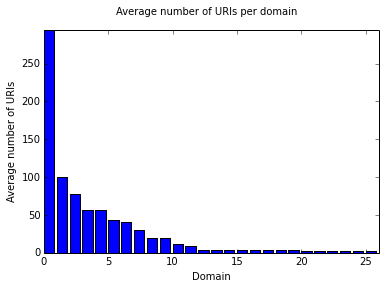
\includegraphics[width=\linewidth]{images/avg_uris_per_domain.png}
  \caption{Average URIs.}
  \label{fig:uris_per_domain:b}
\end{subfigure}
\caption{Number of URIs observed at each domain.}
\label{fig:uris_per_domain}
\end{figure}


\section{Experiment: National Archive Collection}

\begin{enumerate}
\item Get data from major collection
\item BL, archive.org, etc.
\item Apply best strategy from previous section
\item What real-world savings can we demonstrate?
\end{enumerate}

\section{Conclusion}

The defaults in the WARC standard do not take advantage of the fact that many documents on the web will have many minor changes made to them over time. By using a delta algorithm as well as a compression algorithm we can reduce the total archive size by nearly half again.


\end{document}
